\chapter{Revisión de soluciones comerciales}

\section{Gestión de alertas}

La monitorización de la actividad en la red puede ser un trabajo tedioso, sin embargo existen buenas razones pare hacerlo. Por un lado permite buscar e investigar inicios de sesión sospechosos en estaciones de trabajo, dispositivos conectados a redes y servidores mientras identifica las posibles deficiencia de seguridad en la administración del sistema. También puede rastrear las instalaciones software y las transferencias de datos para identificar problemas potenciales en tiempo real en lugar que después de que el daño esté hecho.

El registro, tanto el seguimiento como el análisis debe ser un proceso fundamental en cualquier infraestructura de monitorización. Es necesario un archivo de registro de transacciones para recuperar una base de datos de un desastre. Además, al rastrear los archivos de registro, los equipo de DevOps y los administradores base de datos (DBA) pueden mantener un rendimiento óptimo de la base de datos o encontrar evidencia de actividad no autorizada en el caso de un ciberataque. Por esta razón, es importante monitorizar y analizar regularmente los registro del sistema. Es una forma confiable de recrear la cadena de eventos que condujo a cualquier problema que haya surgido.

Debido a esta serie de problemáticas, existen un número considerable de registro de código abierto y herramientas de análisis disponibles en la actualidad, lo que hace que elegir los recursos adecuados para los registros de actividad sea un trabajo considerable. La comunidad de software de código abierto y gratuito ofrece diseños de registros que funcionan con todo tipo de sitios y prácticamente con cualquier sistema operativo. 

En esta sección se tratará de analizar los productos y herramientas existentes enfocados al tratamiento de log con el fin de averiguar si cumplen con los requisitos planteados o si pueden resultar una ayuda de cara a la implementación de la solución.

\subsection{Graylog}

Graylog comenzó en Alemania en 2011 y ahora se ofrece como una herramienta de código abierto o una solución comercial. Está diseñado para ser un sistema de administración de registros centralizado que recibe flujos de datos de varios servidores o puntos finales y le permite navegar o analizar esa información rápidamente.

Graylog dispone de las siguientes funcionalidades:

\begin{itemize}
\item \textbf{Recolección y procesado de logs}: implemente la necesidad de leer distintos tipos de logs de distintas fuentes para ser tratados de forma descentralizada, así como la posibilidad de integración con directorios LDAP.

\item \textbf{Transformación de datos}: ofrece la posibilidad de transformar los datos de entrada para publicador a otras aplicaciones como fuente de datos refinada.

\item \textbf{Análisis e investigación}: proporciona la capacidad para buscar y analizar información  de distintas fuentes de datos en una única consulta.

\item \textbf{Grafos y estadísticas}: dispone de múltiples gráficos para analizar los datos de forma sencilla accesibles mediante interfaz web.

\item \textbf{Alertas}: provee de la capacidad de crear disparadores y acciones que se activen cuando se produce un evento determinado en los logs. 
\end{itemize}

La arquitectura está compuesta por una serie de nodos que se encargan de leer la información de las máquinas a monitorizar y enviarla a los nodos de Elastic Search que almacenan y procesan todos los logs y mensajes recibidos. Para almacenar los metadatos se utiliza MongoDB y finalmente se proporciona una interfaz web para visualizar los datos recolectados y procesados.


\subsection{Nagios}

Nagios comenzó con un solo desarrollador en 1999 y desde entonces se ha convertido en una de las herramientas de código abierto más confiables para administrar datos de registro. La versión actual de Nagios puede integrarse con servidores que ejecutan Microsoft Windows, Linux o Unix.

Su producto principal es un servidor de registros, cuyo objetivo es simplificar la recopilación de datos y hacer que la información sea más accesible para los administradores del sistema. El motor del servidor de registro de Nagios capturará datos en tiempo real y los enviará a una poderosa herramienta de búsqueda. La integración con un nuevo punto final o aplicación es fácil gracias al asistente de configuración integrado.

Nagios se usa con mayor frecuencia en organizaciones que necesitan monitorizar la seguridad de su red local. Puede auditar una variedad de eventos relacionados con la red y ayudar a automatizar la distribución de alertas. Nagios incluso se puede configurar para ejecutar scripts predefinidos si se cumple una determinada condición, lo que le permite resolver problemas antes de que un humano tenga que involucrarse.

Como parte de la auditoría de red, Nagios filtrará los datos de registro según la ubicación geográfica donde se originan. Eso significa que puede crear paneles de control completos con tecnología de mapeo para comprender cómo fluye su tráfico web.

\subsection{ELK Stack}

\textbf{ELK Stack} o Elastic Stack es un proyecto OpenSource multiplataforma que abarca una serie de productos y soluciones que tienen como finalidad facilitar al usuario el tratamiento de la información. Se trata de una de las herramientas de código abierto más populares entre las organizaciones que necesitan examinar grandes conjuntos de datos y dar sentido a los registros de su sistema. Las funcionalidades básicas serían la de extraer, buscar, analizar y visualizar datos en tiempo real o de forma asíncrona.

ElasticSerch proporciona distintas formas de implementación, tanto de forma local e una única máquina o de forma distribuida utilizando un modelo SaaS (Software as service).

Su oferta principal se compone de tres productos separados correspondientes con sus tres siglas: Elasticsearch, Kibana y Logstash:

\begin{figure}[H]
\centerline{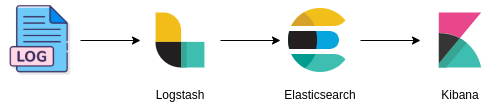
\includegraphics[width=15cm]{figuras/elkstack.png}}
\caption{Componentes del ELK Stack}
\label{enlace1}
\end{figure}

Como breve resumen de los elementos mostrados en la imagen serían:
\begin{itemize}
\item \textbf{Logs:} logs en el servidor que serán analizados e identificados.
\item \textbf{Logstash:} recoge logs y eventos que puede parsear y transformar.
\item \textbf{ElasticSearch:} almacena la información recogida por logstash y la indexa.
\item \textbf{Kibana:} se encarga de explorar, visualizar y compartir los datos almacenados en ElasticSearch.
\end{itemize}

\subsubsection{ElasticSearch}

ElasticSearch es el componente principal de ELK Stack, que presenta como principal responsabilidad las operaciones de catalogar y almacenar información que podrá se recuperada a posteriori de forma flexible. Se trata de un motor de búsqueda OpenSource distribuido y escalable basado en Apache Lucene, que incluye su propio lenguaje de consulta denominado Query DSL. 

Ofrece una API de tipo RESTful Json y clientes para distintos lenguajes de programación de forma oficial, al mismo tiempo que al ser una herramienta OpenSource dispone de una comunidad de usuarios que ofrece clientes y soporte para los lenguajes a los que no se les proporciona oficialmente.

ElasticSearch está compuesto por repositorios, que es donde almacena la información en forma de JSON, en que cada documento es una correlación clave-valor. Su principal objetivo será la de almacenar y catalogar con un índice la información para que sea fácilmente recuperable. Además ofrece interfaces para poder trabajar cond atos de distintas plataformas Big Data como Hadoop y Spark mediante conectores.

\subsubsection{LogStash}

El componente LogStash  se encarga de procesar la información en crudo con el fin de que pueda ser consumida y almacenada por un motor de búsqueda, en concreto en el caso de ELK Stack será ElasticSearch. Se estructura en forma de pipeline con 3 secciones bien diferenciadas:

\begin{enumerate}
\item \textbf{Entrada (input):} conectores e interfaz necesaria para la recepción de datos en crudo de varias fuentes.
\item \textbf{Proceso y filtros (parse):} en esta sección se procesa la información obtenida en un forma comprensible y manejable por un motor de búsqueda. Las transformaciones se basan en filtros con funciones para convertir los datos.
\item \textbf{Salida (output):} conector de salida de la información procesada tras el filtrado. Por defecto la salida será ElasticSearch pero ofrece conexiones para otras plataformas.
\end{enumerate}

\subsubsection{Kibana}

El elemento restante del stack es Kibana, que proporciona la interfaz gráfica con la función de monitorizar. Se encarga de leer la información de ElasticSearch para después presentarla a través de una interfaz web donde se visualizará el contenido almacenado en el motor de búsqueda.

Dispone de gran variedad de gráficas, métricas histogramas y visualizaciones configurables que permiten analizar la información. Se basa en node.js y se trata de un cliente web multiplataforma OpenSource que podrá ser ejecutada en multitud de plataformas.


\subsection{Conclusiones}

Las herramientas mencionadas en esta sección proporcionan parte de la funcionalidad que se busca con este proyecto, sin embargo no consiguen todos los objetivos propuestos. Esto no quita que se pueda utilizar parte de la funcionalidad propuesta por la herramienta con el fin de construir la solución final del proyecto. Tras el análisis realizado de posibles herramientas utilizadas en el mercado se ha decidido eliminar GrayLog ya que se parte del requisito de que la solución deberá utilizar productos OpenSource, y en este caso la licencia gratuita de GrayLog solo permite el tratamiento de 2 GB diarios, lo cual no es lo suficiente para una aplicación como sobre la que va a actuar la solución. Por otro lado, Nagios no dispone de una licencia OpenSource y se descarta por este motivo.

Finalmente se ha optado utilizar por una de ellas, concretamente ELK debido a la extensa documentación y comunidad, así como su posibilidad de escalado y a la rapidez de búsqueda gracias al indexado de la información. Utilizando las últimas versiones de kibana se podría utilizar las herramientas de gestión de alertas para la generación de eventos, sin embargo, esto no entra dentro de la licencia OpenSource y los triggers que dispone son limitados. 

Debido a que existe una gran comunidad de usuarios de Elastic Search, existe una comunidad dedicada a la creación de plugins y complementos que mejoran el uso y proporcionan herramientas que con la herramienta de stock no dispondríamos. Gracias a ello para la gestión de alertas se podrá utilizar la herramienta ElastAlert, que se trata de una herramienta totalmente Open Source creada como complemento a Kibana para suplir las limitaciones presentes a la hora de alertar sobre incoherencias.

De esta forma aun teniendo que emplear tiempo en el conocimiento de las funcionalidades de la herramienta, será más eficiente que desarrollar una herramienta desde 0. Así se podrá asignar mas tiempo a las posibilidades de parametrización de la solución para poder ser aplicada a otros proyectos y en otros entornos.

